\chapter{Lehmanns-Gesetze}
\label{chapter2}
In diesem Kapitel wird auf Lehmanns Gesetze eingegangen. Hierbei werden zunächst die Personen Lehmann und Bélády betrachtet.\\
Anschließend werden das erste und zweite der Gesetze von Lehmann und Bélády erläutert. Mit diesem Wissen können einige inneren und äußeren Ursachen für Lehmanns Gesetze analysiert werden.\\
Das Kapitel schließt mit den langfristigen Auswirkungen von Lehmanns Gesetzen. 

\section{Die Personen Lehmann und Bélády}
Die Zusammenhänge zwischen Benutzung und Anpassung der Software wurden schon früh in der Informatik erkannt. Der Informatik-Professor Manny Lehman und der Informatiker László Bélády formulierten zwischen 1974 und 1996 eine Reihe von Gesetzen. Diese nannten sie die “Laws of Software-Evolution“. Die Gesetze beschreiben ein Gleichgewicht zwischen Kräften, die neue Entwicklungen vorantreiben, auf der einen Seite und Kräften, die den Fortschritt bremsen, auf der anderen Seite. \cite{lehman_understanding_1979}

\subsection{Korrektheit von Lehmanns Gesetzen}
Lehmanns und Bélády’s Gesetze sind weniger Gesetze, als es Beobachtungen sind. Die Korrektheit dieser Beobachtungen wurde bereits in vielen Systemen und Anwendungen untersucht und validiert.\\
Ein Beispiel dafür wäre die Arbeit von Feitelson et al. \cite{israeli_linux_2010}. In dieser wurden 810 Version des Linux-Kernels, welche über ein Zeitraum von 14 Jahren veröffentlicht wurden, nach der Evolution des Software-Systems charakterisiert. Als Basis wurden Lehmanns Gesetze angenommen und diese mit verschiedensten Metriken nachgewiesen. \\
Zum Beispiel wurde das System-Wachstum anhand von Codezeilen oder der Anzahl von Funktionen quantifiziert. Darüber hinaus wurde das funktionale Wachstum von Linux anhand der Anzahl von Systemaufrufen gemessen.\\
Dabei konnten das erste und zweite von Lehmanns Gesetzen nachgewiesen werden. Auf diese wird im Folgenden eingegangen.

\subsection{Das erste und zweite Gesetz}
Lehmann und Bélády haben im ersten Gesetz schon 1974 erkannt, dass eine Änderung und Umstrukturierung eines Software-Systems stattfindet. Vorausgesetzt das Software-System wird aktiv genutzt. Ferner wurde im zweiten Gesetz erkannt, dass der Effekt dieser Änderung negativ ist. Außer es wird ein zusätzlicher Aufwand unternommen, um dem entgegenzuwirken.
\pagebreak

\section{Gründe für Lehmanns Gesetze}
Nachdem Feitelson et al. die Gültigkeit von Lehmanns Gesetzen festgestellt hat, gilt es zu fragen, warum diese Gesetze gelten. Ausgangspunkt dafür sind äußere und innere Kräfte, welche auf die Software einwirken.\\
Auf diese beiden Kräfte wird im Folgenden eingegangen.

\subsection{Äußere Gründe für Lehmanns Gesetze}
Ein Softwaresystem ist nicht isoliert zu betrachten. Es ist in eine Umgebung eingebettet. Grundsätzlich besteht ein Bedarf an Anpassungen, wenn sich die Umgebung der Software wandelt.\cite{bommer_softwarewartung_2016} Hierfür werden im Folgenden einige mögliche Gründe aufgeführt:

\begin{itemize}
    \item Beispiel für die fachliche Umgebung einer Software wären neue Compliance-Anforderungen. Wird eine Software über viele Jahre oder Jahrzehnte genutzt, sind Gesetzesänderungen zu erwarten. Folglich muss eine, sich in der Benutzung befindende, Software darauf reagieren.
    \item Auch ein Umdenken in der Geschäftsstrategie ist ein möglicher äußerer Faktor. Neue Märkte haben neue Anforderungen. Ein Beispiel hierfür wäre das Expandieren nach China. Im fern-östlichen Raum gelten nicht nur andere Gesetze, sondern auch andere Sitten. Dies kann umfangreiche Änderungen an der Software nach sich ziehen.
    \item Darüber hinaus kann auch ein neues Vertriebsmodell für Veränderung sorgen. Beispiele hierfür wären Geschäftsmodelle wie \ac{SaaS}. Auf \acs{SaaS} wird im Rahmen des letzten Kapitels umfangreicher eingegangen.
    \item Abschließend kann auch ein Fortschritt der Technik Auslöser für eine Reihe von neuen Anforderungen sein. Neue Programmiersprachen und Frameworks können ein schnelleres Voranschreiten in der Entwicklung ermöglichen. Letzteres wiederum kann so die Zeit zwischen der Entwicklung und dem ersten Release verkürzen. Auch Fehler im System können möglicherweise schneller behoben werden. Sollte die Konkurrenz die genannten Vorteile erzielen, kann dies ein Wettbewerbsvorteil für die Konkurrenz sein.
\end{itemize}

\subsection{Innere Gründe für Lehmanns Gesetze}
Neben den bereits beschriebenen äußeren Einflüssen führen auch eine Reihe von inneren Gründen zu Lehmanns Gesetzen. Die Software erfährt auch ein Wandel der technischen Umgebung. Im Folgenden werden hierfür einige Beispiele angeführt:

\begin{itemize}
    \item Seacord et al. \cite{seacord_modernizing_2003} führt als ersten Grund Verbesserungen an dem Produkt selbst an. Hierzu gehört Fehlerverbesserungen und Performance-Optimierungen. Neue Komponenten werden hinzugefügt, existierende Komponenten angepasst. \cite{seacord_modernizing_2003}
    \item Während der Definitions-Phase der Architektur kann ein Grad von Anpassungsfähigkeit und Flexibilität eingeplant werden. Jedoch sind nicht die Anforderungen bekannt, welche erst in der Zukunft gestellt werden. Die Architektur kann nicht für diese ausgelegt werden. Folglich degeneriert die Architektur zunehmend.\cite{seacord_modernizing_2003}\cite{daniel_kramer_legacy-software_2020}
    \item Darüber hinaus wächst die Code-Basis. Wiederholte Modifikation führt meist zu mehr Code und komplexerer Software. Das System wird folglich brüchiger. Die Wahrscheinlichkeit von Seiteneffekten nimmt zu, mit jeder Änderung die eingearbeitet wird. Die Wartung der Software wird folglich Schritt für Schritt schwieriger. Letzteres verlangt nach mehr Personal und nach speziell geschulten Personal. \cite{seacord_modernizing_2003}\cite{daniel_kramer_legacy-software_2020}
    \item Abschließend ist es möglich, dass neue Mitarbeiter an der Software arbeiten. Die ursprünglichen Mitarbeiter, welche die Architektur der Software entwickelt haben, sind möglicherweise nicht mehr in der Firma beschäftigt oder im Ruhestand. Spätestens jetzt können Verständnisprobleme mit der Definition der Architektur oder der bestehenden Code-Basis aufkommen.\\
    Fehlende Dokumentation, gealterte Programmiersprachen oder das Missachten von Programmierrichtlinien in der Vergangenheit verstärken diesen Effekt. \\ 
    Seit 1970 sind die Kosten für die Wartung so weit gestiegen, dass sie die Kosten der initialen Entwicklung übersteigen. Grafik \ref{fig:costsOfModernization} verdeutlicht dies.
\end{itemize}

\begin{figure}[h] 
  \centering
  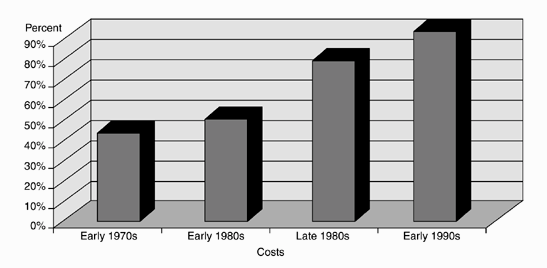
\includegraphics[width=0.7\textwidth]{Chapters/2-Lehmanns-Gesetze/images/costsDevotedToSoftwareModernization.png}
  \caption{Software-Kosten, welche der Software-Modernisierung gewidmet werden. \cite{seacord_modernizing_2003}}
  \label{fig:costsOfModernization}
\end{figure}

\pagebreak

\section{Langfristige Auswirkungen von Lehmanns Gesetzen}
Wird das System nicht an die gewandelte Umgebung angepasst, entsteht zunehmen eine Diskrepanz zwischen der Umgebung der Software und dem Softwaresystem selbst. Grafik \ref{fig:fehlendeVerbesserung} illustriert diesen Zusammenhang.\\
Fehlt den Mitarbeitern das Verständnis für die Architektur und bestehende Codebasis, wird es zunehmend schwieriger die Software anzupassen. Möglicherweise ist die Software nicht umfassend testbar. 
Änderungen können folglich unvorhergesehene Wechselwirkungen hervorrufen. \cite{daniel_kramer_legacy-software_2020} \\
Dies führt unter den Mitarbeitern zu dem sogenannten “Fear-Driven-Development“\cite{daniel_kramer_legacy-software_2020}. Anpassungen werden dadurch nur spärlich eingearbeitet und meist vermieden.\\  
Die Software wird demnach resistent gegen Änderungen am Code. Eine Erhaltung oder Steigerung der Effizienz setzt allerdings Änderungen voraus. 
Darüber hinaus sind Fehlerursachen ohne umfassende Kenntnisse der Codebasis schwieriger auszumachen. Die Zeit und Kosten Fehler zu beseitigen steigen.\\
Zusammenfassend lässt sich also sagen, dass die Software unwirtschaftlicher wird. Immer größere Investitionen werden nötig um immer weniger Steigerungen in der Nützlichkeit der Software zu erreichen. Folglich wird die Software von Konkurrenz-Produkten überholt und zunehmend weniger konkurrenzfähig.
\begin{figure}[bth] 
  \centering
  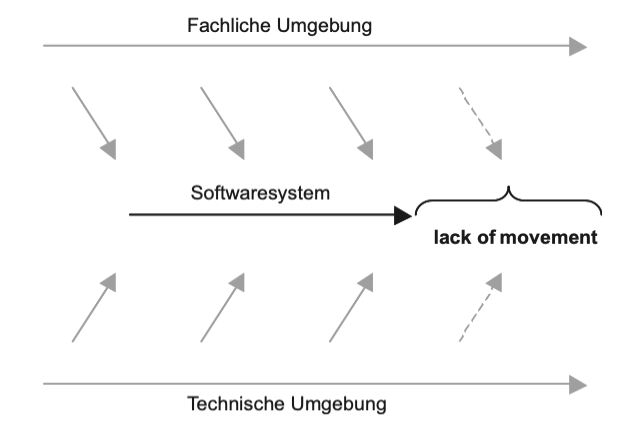
\includegraphics[width=0.7\textwidth]{Chapters/2-Lehmanns-Gesetze/images/fehlendeVerbesserung.png}
  \caption{Folgen einer fehlenden Anpassung der Software an ihre Umgebung \cite{bommer_softwarewartung_2016}}
  \label{fig:fehlendeVerbesserung}
\end{figure}

\section{Zusammenfassung}
Zusammenfassend lässt sich sagen, dass sich die Problemstellung der Software-Alterung auf zwei verschiedene Aspekte bezieht.\\
Zunächst wird durch Lehmanns Gesetze klar, dass eine Software angepasst werden muss. Sonst schreitet das Umfeld der Anwendung fort, während die Anwendung stehen bleibt. Die Software veraltet. Führt man allerdings Änderungen an der Software durch Ergeben sich neue Probleme. Denn werden die Grundprinzipien der Architektur missachtet, degeneriert die Architektur. Diese Degeneration führt erneut zu einer Alterung der Software. Folglich stellt sich die Frage, wie dieser Alterung entgegengewirkt werden kann, ohne die Architektur zu schädigen.




